\documentclass[12pt,a4paper]{article} %aqui fala o tipo de documento e o 
tamanho da fonte. Opções: tamanho do texto (10pt, 12pt, 14pt), formato 
do papel (a4paper, a5paper, b5paper, letterpaper, legalpaper, 
executivepaper), o número de colunas (onecolumn, twocolumn), entre 
outras opções.
%Por exemplo, [12pt,a4,twocolumn].
%classe: article, report, letter, book ou slides. Instalar abnt para 
quem está pensando no tf
\usepackage{indentfirst}
\usepackage[brazil]{babel} %hifenização em português do brasil
\usepackage{listings}
\usepackage[T1]{fontenc} % caracteres com acentos são considerados um 
bloco só
\usepackage{ae} %arruma a fonte quando usa o pacote acima
\usepackage[utf8]{inputenc}
\usepackage{graphicx}%Para inserir figuras
\usepackage{color}
 
\definecolor{codegreen}{rgb}{0,0.6,0}
\definecolor{codegray}{rgb}{0.5,0.5,0.5}
\definecolor{codepurple}{rgb}{0.58,0,0.82}
\definecolor{backcolour}{rgb}{0.95,0.95,0.92}
 
\lstdefinestyle{mystyle}{
    backgroundcolor=\color{backcolour},   
    commentstyle=\color{codegreen},
    keywordstyle=\color{magenta},
    numberstyle=\tiny\color{codegray},
    stringstyle=\color{codepurple},
    basicstyle=\footnotesize,
    breakatwhitespace=false,         
    breaklines=true,                 
    captionpos=b,                    
    keepspaces=true,                 
    numbers=none,                    
    numbersep=5pt,                  
    showspaces=false,                
    showstringspaces=false,
    showtabs=false,                  
    tabsize=2    
}
 
\lstset{style=mystyle}
\begin{document} % Aqui começa o documento
\title{Tutorial RS-232 da placa DE2-115 da Altera\vspace{3.5cm}} % 
título
\author{
	Gustavo de Faria Silva - 
	\texttt{gustavofaria@ufu.br}
	\and
	João Paulo de Oliveira - 
	\texttt{joaopaulodeoliveira123@gmail.com}
	\and
	Lucas Rossi Rabelo - 
	\texttt{lucasrossi98@hotmail.com}
	\vspace*{11.6cm}
}

% * <joaopaulodeoliveira123@gmail.com> 2017-11-23T13:53:11.198Z:
%
% ^.
\maketitle %cria o título
\thispagestyle{empty}
\pagebreak
%\def \negritovi {\textbf} %Criando comandos

\tableofcontents %índice
\thispagestyle{empty}
\pagebreak % Quebra de página
%\listoffigures %indice de fig%uras
%\listoftables %indice de tabelas
%\pagebreak % Quebra de página
\section{Introdução}
O trabalho tem como objetivo mostrar como é feita a comunicação entre a 
DE2-115 e um computador de propósito geral. O material mostra o 
adaptador utilizado, bem como uma demonstração do hardware responsável 
pela troca de dados, algumas características da placa, além de mostrar o 
passo a passo da configuração no computador e no final é feita uma 
demonstração através de um exemplo do envio de caracteres em ASCII da 
DE2-115 para o computador através do PUTTY.

\section{Caracteŕisticas físicas e elétricas}
O RS-232 na Placa DE2-155 da Altera oferece um conector DB-9 fêmea para 
fazer o interfaceamento com o computador ou outro dispositivo de 
comunicação. Um computador conectado com a placa deve ter as seguintes 
configurações\cite{man}
\begin{itemize}
	\item \bf{Taxa de transferência:} 115200
    \item \bf{Bit de paridade:} Nenhum
    \item \bf{Bits de dados:} 8
    \item \bf{Bit de parada:} 1
    \item \bf{Controle de fluxo:} ON
\end{itemize}
A DE2-115 usa o transceptor ZT3232 para gerenciar a conexão entre a 
placa. Para mais detalhes sobre o transceptor, consulte o datasheet. 

\begin{figure}[!htb]
\centering
	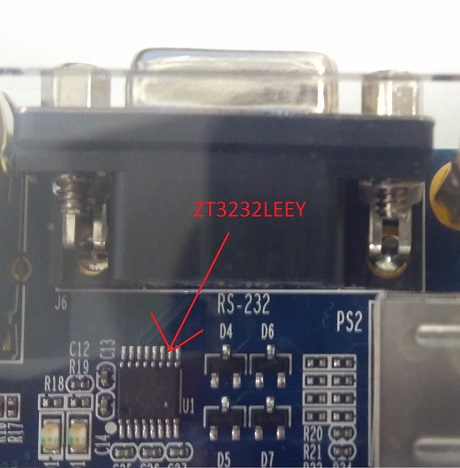
\includegraphics[scale=0.5]{imagens/IMG_20171123_110859}
	\caption{CI utilizado para o RS-232}
	\label{CI}
\end{figure}
A pinagem é conectada ao FPGA da seguinte forma:
\begin{figure}[!htb]
	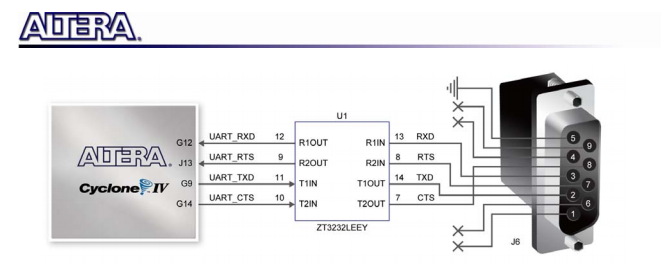
\includegraphics{imagens/conexo.png}
	\caption{Pinagem utilizada entre o FPGA e o ZT3232LEEY}
	\label{Conexao}
\end{figure}

\begin{table}[!htb]
\centering
\caption{Tabela de associação de pinos}
\label{pin_assignment}
\begin{tabular}{|l|l|l|l|}
\hline
\textbf{Pino} &\textbf{No Pino FPGA} & \textbf{Descrição} & 
\textbf{Voltagem} \\ \hline
RXD         & PIN\_G12    & Receptor da UART               & 3.3V     \\ 
\hline
TXD         & PIN\_G9     & Transmissor da UART            & 3.3V     \\ 
\hline
CTS         & PIN\_G14    & Limpar para enviar na UART     & 3.3V     \\ 
\hline
RTS         & PIN\_J13    & Requisição para enviar na UART & 3.3V     \\ 
\hline
\end{tabular}
\end{table}

A conexão será feita através do adaptador RS-232 <-> USB mostrado na 
figura 3:

\begin{figure}[!htb]
\centering
	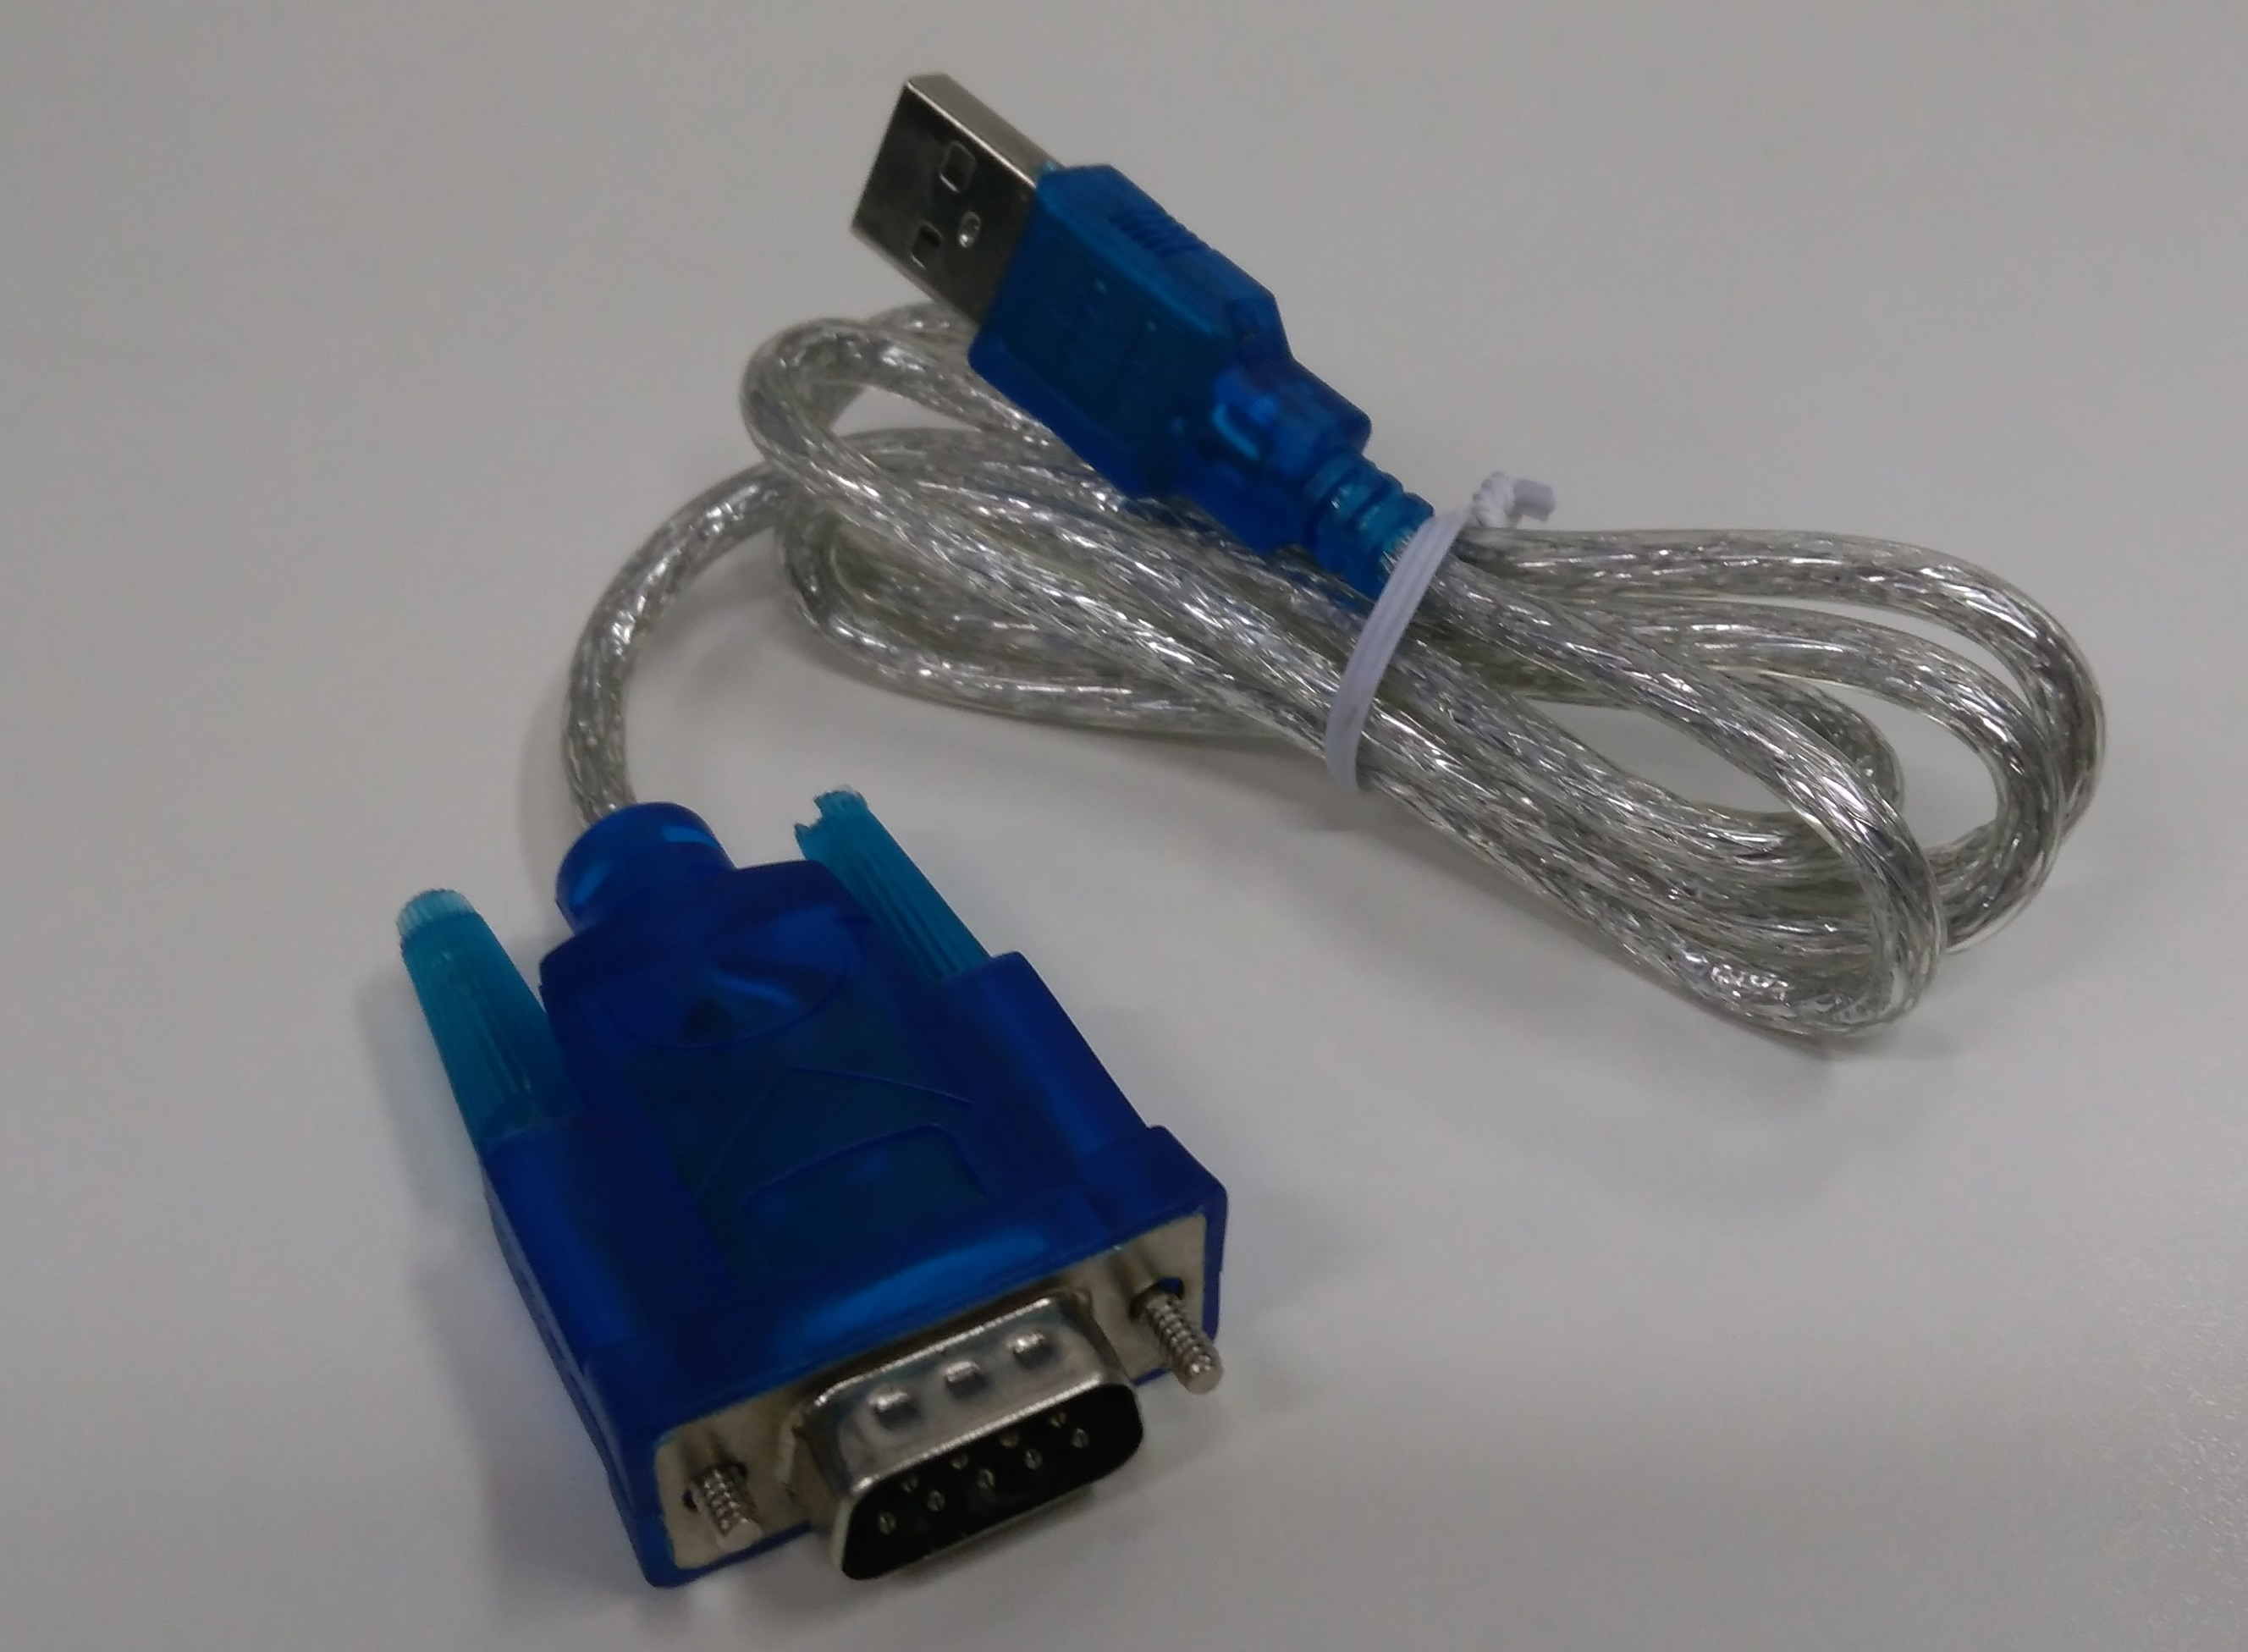
\includegraphics[scale=0.06]{imagens/adaptador.jpg}
	\caption{Adaptador utilizado para a comunicação}
	\label{Adaptador}
\end{figure}

\section{Interfaceamento}
O PUTTY é um emulador de terminal e emulador serial que suporta vários 
protocolos de internet incluindo SPC, SSH, TELNET, rlogin e conexão de 
soquete bruto. Além disso, faz conexão com a porta serial. Ele é 
suportado por Windows e Linux.

Para começar, deve-se configurar a porta serial da máquina para que o 
PUTTY consiga fazer a comunicação, deve-se descobrir a porta COM em que 
o conversor USB/RS-232 foi conectado. No Windows isso pode ser 
facilmente verificado no gerenciador de dispositivos, nos controladores 
USB como destacado na imagem.

\begin{figure}[!htb]
\centering
	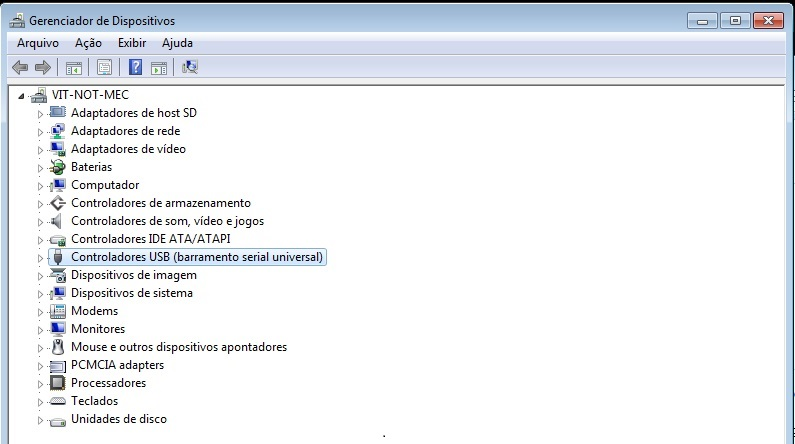
\includegraphics[scale=0.7]{imagens/289124.jpg}
	\caption{Gerenciador de dispositivos}
\end{figure}
Suponha que o nosso Adaptador está na porta COM4, assim devemos 
configurar o PUTTY para serial como mostra na Figura 5. Essa tela de 
configuração é exibida na inicialização do PUTTY.
\begin{figure}[!htb]
\centering
	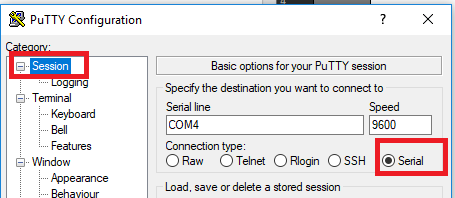
\includegraphics[scale=0.6]{imagens/config1.png}
	\caption{Configuração na aba Session no PUTTY}
	\label{config1}
\end{figure}


\pagebreak
A única configuração necessária nessa aba é selecionar a comunicação 
serial como destacado na imagem acima.

Na aba serial, devemos utilizar as configurações mostradas na seção 1. 
Na figura 6, foi configurado exatamente para a DE2-115 e a porta COM4. 
Note que a taxa de transferência foi configurada para 9600 considerando 
o exemplo presente na seção 3.1, nele, o clock é dividido para resultar 
em uma taxa de transferência de 9600.

\begin{figure}[!htb]
\centering
	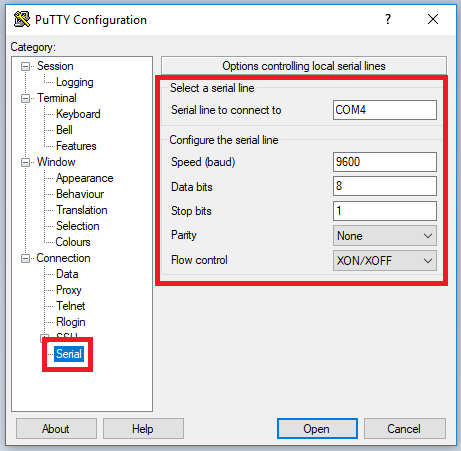
\includegraphics[scale=0.6]{imagens/config2}
	\caption{Configuração na aba Session no PUTTY}
	\label{config2}
\end{figure}
Feito isso, podemos iniciar abrir a comunicação com a DE2-115 clicando 
no botão Open, daí será aberto o terminal de comunicação do PUTTY.

Resta agora programar a placa para fazer a comunicação. Veja o exemplo:

\subsection*{Exemplo}

O código a seguir está na linguagem System Verilog e pode ser gravada na 
placa através do Quartus II, no código está descrito uma máquina de 
estado finito que efetua o envio de 1 byte de dados, que é recebido pelo 
PUTTY na forma de carácter na tabela ASCII.

O exemplo está mapeado para a placa DE2-115 com os assignments 
disponibilizados pela Altera. As entradas e saídas utilizadas são 
\cite{Baker}
\begin{itemize}
	\item \textbf{SW:} As chaves de 0 até 7 serão mapeadas para o 
byte a ser enviado.
	\item \textbf{KEY:} São os botões 0 e 1 na placa:
	\begin{itemize}
		\item \textbf{KEY0:} Corresponde ao Clock da placa. 
Quando pressionado, a placa envia o carácter representado nas chaves, 
porém, não é feito o debounce, então quando pressionado, pode ocorrer o 
envio de vários caracteres com um único clique.
		\item \textbf{KEY1:} Corresponde ao reset da 
comunicação.
	\end{itemize}
	\item \textbf{UART TXD:} É a saída serial do conector DB-9 da 
placa.
\end{itemize}
\lstinputlisting [language=verilog]{Codigo/rs232.sv}
\pagebreak
\bibliographystyle{plain}
\bibliography{refs}
\end{document}
